\subsection{Filter Distribution}\label{q:Filters}

The Phase 1 SCOC report recommended implementing a single exposure for $u$ band visits (see \citetalias{PSTN-053} Q3), and maintaining overall visit times of 30 seconds for all other bands instead of variable visit (or exposure) times. Specific questions concerning filter balance, particularly considering a bluer skew of the survey (see \citetalias{PSTN-053} Q4), and more consideration of varying exposure time per visit were left to be addressed in Phase 2 report with the support of v2.X simulations. The specific questions to be addressed in the Phase 2 SCOC deliberations include:



\begin{enumerate}
\item Should the survey strategy skew towards bluer filter observations compared to the current baseline (bluer here is in reference to \texttt{baseline\_v1.7} and includes the consideration of additional coverage in either $u$ or $g$ bands)?
\item Should the same filter balance be applied to the entire LSST footprint (as opposed to, for example, implementing different filter balance in the extragalactic \emph{vs.} Galactic sky)?
\item What should the exposure time be for the $u$-band observations (including considerations of extending the $u$ band exposures to 50 seconds)? 
\item Should the survey use variable visit times or a set exposure time in each filter?
\item Should the survey use a different exposure than 2x15s (or possibly 1x30s) for non-$u$-band filters (for example, as implemented in the \texttt{shave\_filters\_v2.1} simulations)?
\end{enumerate}

\subsubsection{SCOC recommendations: executive summary }\label{rec:filterdist_es}

The SCOC has converged on most recommendations relating to filter distribution and has answered the questions left open in the Phase 1 report with the guidance of the reports and metrics provided by the community. Results on relevant metrics are included in a comparison notebook purposefully designed by the Survey Strategy team to guide filter-balance consideration\footnote{\url{https://github.com/lsst-pst/survey_strategy/blob/main/fbs_2.0/Filter\%20Balance.ipynb}.}. {\bf The SCOC recommends to retain the filter balance and visit/exposure times as implemented in \texttt{baseline\_v2.X} on the WFD and tentatively in the Galactic Plane and Bulge, and SCP, although additional refinements on these and other minisurveys and special regions should continue to be considered.}

\subsubsection{SCOC recommendations: point by point answers }\label{rec:filterdist}

\begin{enumerate}

\item The SCOC recommends that the WFD filter balance implemented in \texttt{baseline\_v2.1}  be maintained in the low-dust WFD survey.\footnote{The depth by filter as implemented in simulation \texttt{baseline\_v2.0} is reported in \citep{PSTN-054} Table 3. The filter balance is essentially unchanged since \texttt{baseline\_v1.7}.} Skewing the WFD survey strategy towards bluer filter observations would harm several science cases while providing benefits only to a few. 
SSSC and DESC science do not favor bluer filter observations (as presented in their reports).
The filter balance notebook\footnote{
\url{https://github.com/lsst-pst/survey_strategy/blob/main/fbs_2.0/Filter\%20Balance.ipynb}.
} shows no strong support for a blue skew among the TVS metrics and indicates detrimental effects for cadence-dependent DESC metrics and SSSC metrics (examples of relevant SSSC metrics include Fraction LC inversion PHA H=16.0 and 19.0, Fraction LC inversion NEO H=16.0 and 19.0, Fraction LC inversion MBA H=16.0 and 18.0, Fraction LC inversion Trojans H=14.0 and 15.0). The v3.0 baseline implements this recommendation with the following ratios of median number of images in the WFD, compared to $r$ band: ($u$, $g$, $r$, $i$, $z$, $y$) $\sim$ (0.25, 0.35, 1.0, 1.0, 0.87, 0.90)


\item Conversely, although Galactic TVS science does not favor blue-enhanced $u$ and $g$ coverage, as it causes a detrimental decrease in performance for almost all regions,  different minisurveys as well as the Galactic Plane may benefit from changes to the default balance. \emph{The SCOC is not ready to produce a final recommendation for the filter balance for the Galactic Plane/Bulge or SCP region - we will continue working with the SMWLV and TVS SCs to find the best filter balance for Galactic science (see also \autoref{q:Footprint}).}

\item There is no evidence for significant performance improvements with either increased or variable $u$-band visit exposure length. We, therefore, recommend that the $u$-band 30 second exposure time implemented as a single 1x30s exposure visit so as to avoid becoming read-noise dominated \citep{PSTN-053},  be preserved.

As the basis for this conclusion, the SCOC considered several factors.  The reports from the SSSC disfavor the \texttt{long-$u$} simulation family. Simulations with the same number of $u$ visits as the \texttt{baseline\_v2.1} but a 50s exposure time showed enhanced results for X-ray binaries, the Galactic Bulge, and pencil beam fields in the $u$-band, but at the expense of observations in the other filters which are more important for most galactic transient science, which therefore does not overall favor longer or variable-length $u$ exposures. Increased $u$-band might lead to the enhanced discovery of new transient  extragalactic objects but may disfavor studies of kilonovae which are expected to be red in color (as reported in the TVS SC extragalactic science report).

The \texttt{long\_u2} simulations increase the exposure time for visits in $u$ without decreasing the overall number of $u$ visits, but at the expense of other bands, and this family of strategies is not strongly preferred by any science case reviewed by this committee.

\item There is no evidence for significant overall improvements by varying the exposure time (for example in response to observing conditions). In light of the additional expected complications in calibration and time-variability analysis if variable exposure times are introduced, the SCOC recommends against dynamically varying the exposure time. 

\item Conversely, the SCOC recommends revisiting the exact exposure length in each filter once the performance of the system-as-built is ascertained: it is possible that rebalancing the exposure time to compensate for performance and throughput in some filters as compared to others or shortening exposures in filters where the throughput exceeds expectations, enabling the collection of more images in that filter (or overall), could lead to enhanced LSST science. \emph{The SCOC cannot finalize this recommendation at this time due to missing information about the characteristics of the system-as-built}.

%\item The SCOC recommends against $u-$band observations longer than 30\,s, as implemented in the \texttt{baseline\_v2.1}.

%The reports from the SSSC disfavour the \texttt{long-$u$} simulation family. Simulations with the same number of $u$ visits as the \texttt{baseline\_v2.1} but a 50s exposure time showed enhanced results for X-ray binaries, the Galactic Bulge, and pencil beam fields in the $u$-band, but at the expense of observations in the other filters which are more important for most galactic transient science, so this is not preferred. Increased u-band might lead to enhanced discovery of new transient  extragalactic objects, but may disfavor studies of kilonovae which are red (as reported in the TVS SC analysis).

%The \texttt{long\_u2} simulations that increase the exposure time for exposures in $u$ without decreasing the overall number of $u$ exposures may be a fair compromise, but it is not strongly preferred by any science cases reviewed by this committee.

\end{enumerate}
\begin{figure*}
    \centering
    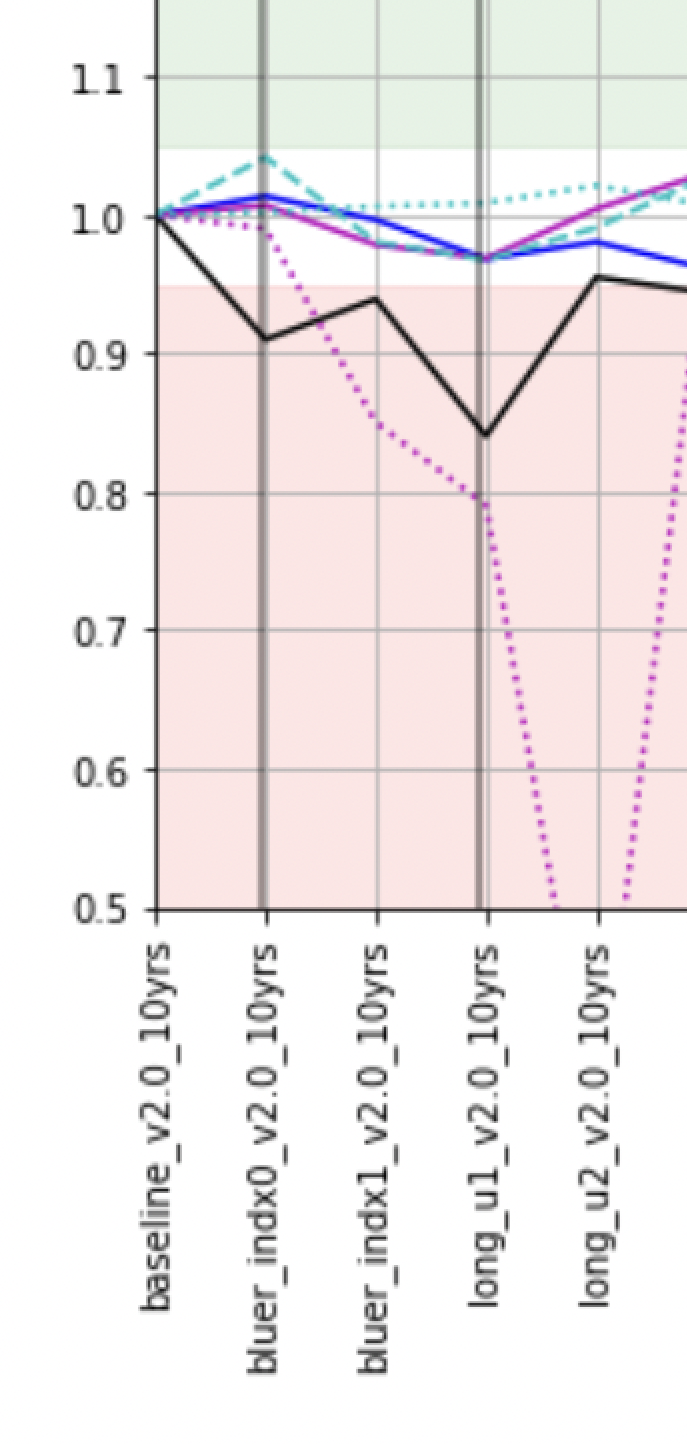
\includegraphics[width=1.7in]{figures/Filter_2.png}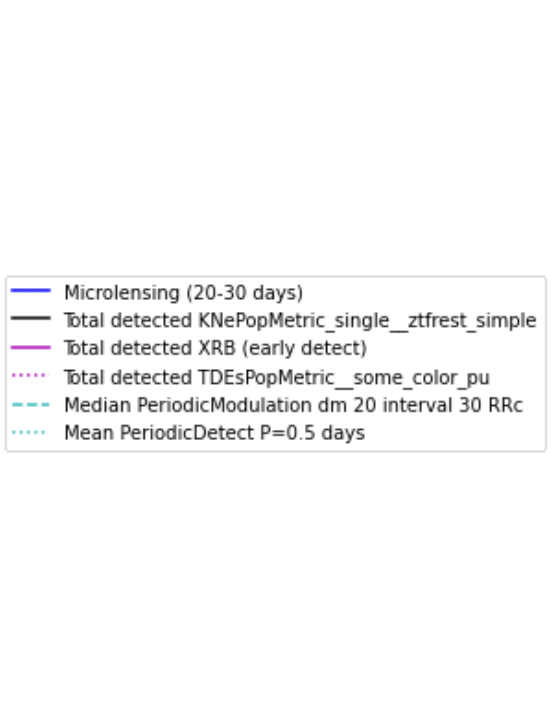
\includegraphics[width=2.5in]{figures/Filter1_Label.png}
    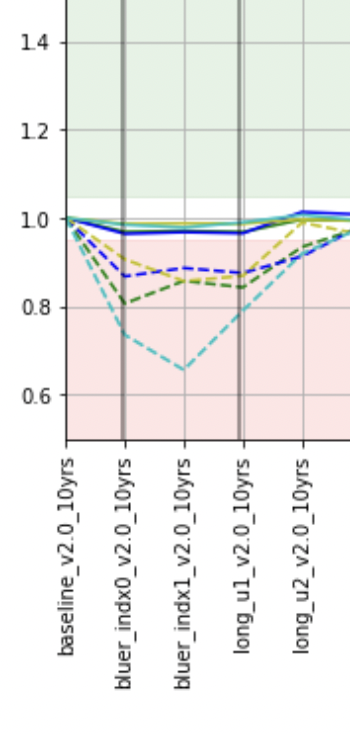
\includegraphics[width=1.7in]{figures/Filter_1.png}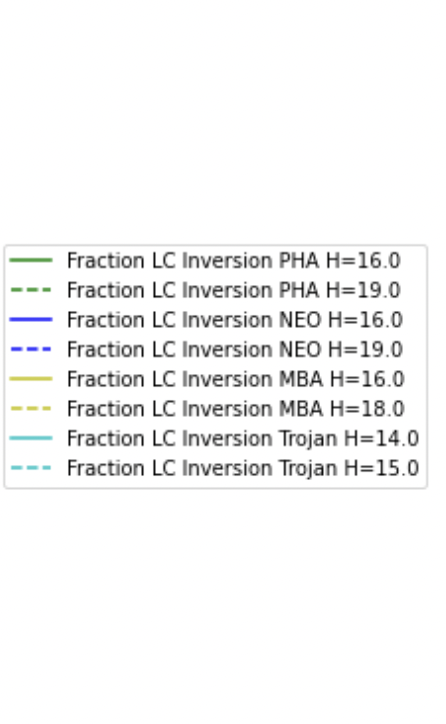
\includegraphics[width=2.3in]{figures/Filter2_Label.png}
    \caption{Impact of skewing the filter balance toward bluer filters for time-domain science metrics provided by the TVS SC (\emph{top}) and Solar System metrics provided by the SSSC (\emph{bottom}). The first point on the $x$ axis represents the benchmark performance of \texttt{baseline\_v2.0}, all simulations to the right of that skew toward bluer surveys by either increasing the fraction of observations in $u$ band or by increasing the length of the $u$ band exposures. In most cases the metrics are neutral or respond negatively to bluer implementations of LSST. The negative impact can be as significant as a 60\% drop in metric performance.}\label{fig:filterF1}
\end{figure*}
In addition, after the November 2022 SCOC workshop,\footnote{\url{https://project.lsst.org/meetings/scoc-sc-workshop3/home}.} a request was made by the community (in particularly by members of the DESC) to make the $z$  filter more often available for observation: the Rubin Observatory filter wheel can house 5 of the 6 Rubin filters on any given night. The default plan as implemented in the v2.X simulations has been to swap $u$ and $z$ bands according to the moon phase. Availability of $z$ on the filter wheel on more nights produces smaller time gaps in the DDF observations (see \autoref{q:DDF}) in a wavelength range important for the characterization of high redshift SNe, with improved throughput for SN Ia cosmology. To support the DESC request simulations were made with the $u, z$, and $y$ filters alternating on the filter wheel. This minimally impacts filter balance but does impact the median time gaps for multiple filters as discussed in \autoref{q:Visits}. \emph{The SCOC recommends to continue the investigation of filter swap options while overall respecting the SCOC recommended filter balance}. 
